\section{POSIX Threads Programming}

Für UNIX Systeme steht ein stardardisiertes threads programming interface in C zur Verfügung (POSIX threads / pthreads).


\subsection{UNIX Process vs. UNIX Thread}

\begin{center}
    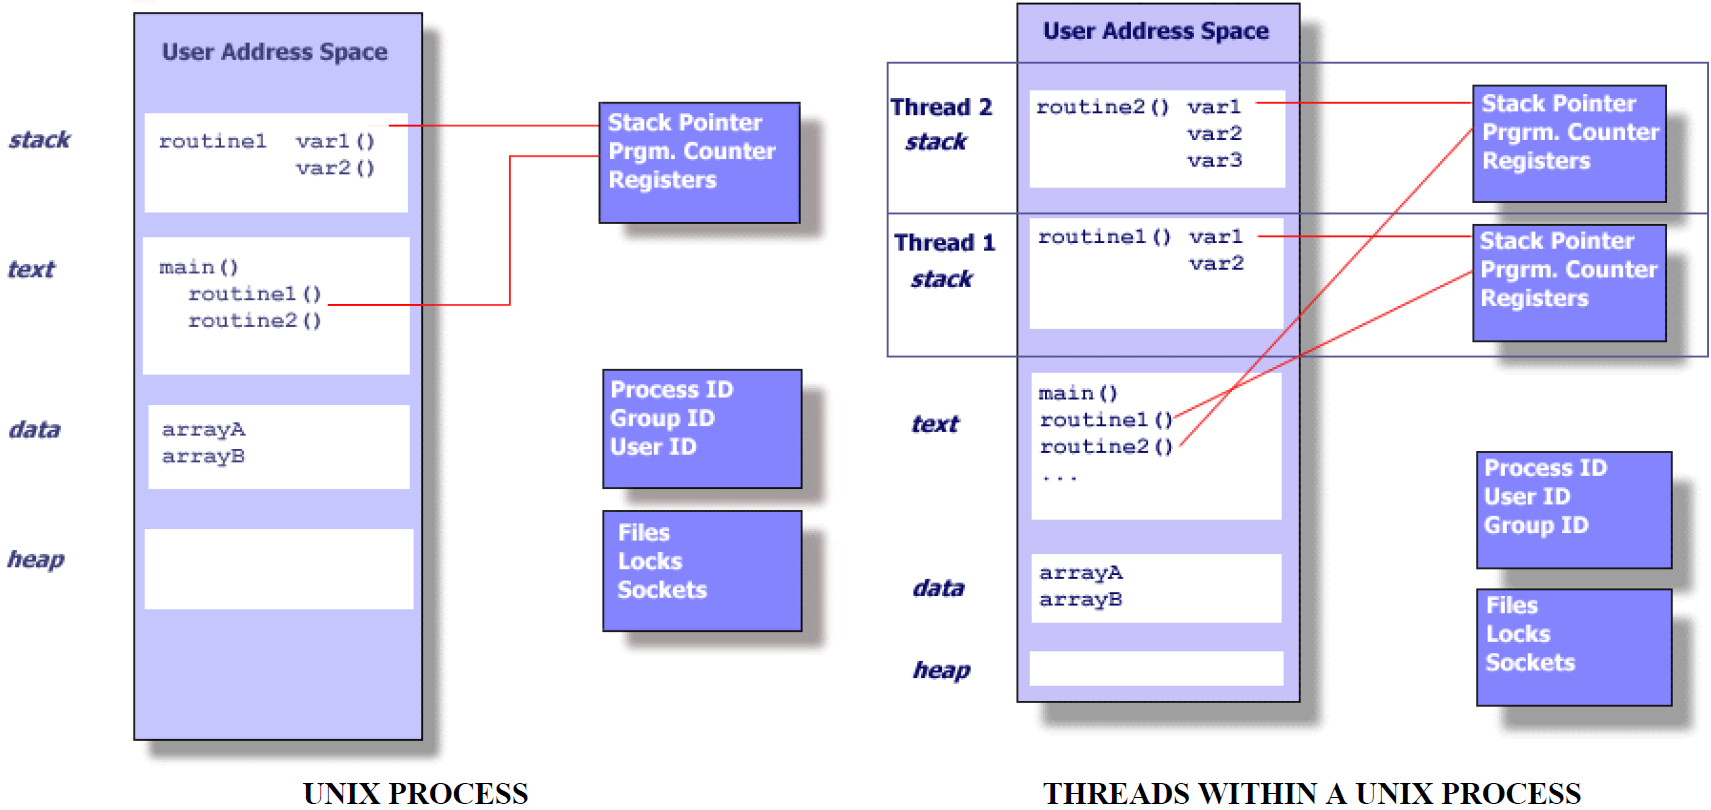
\includegraphics[width=0.75\columnwidth]{images/posix_process_threads.png}
\end{center}


\subsubsection{UNIX Process}

\begin{outline}
    \1 \textbf{heavyweight process} (generiert von Betriebssystem)
    \1 Prozess erfordert \textbf{erheblichen overhead}, da Informationen über Programmressourcen und 
        den Ausführungsstatus des Programms, beispielsweise:
        \2 Prozess-ID, Prozessgruppen-ID, Benutzer-ID und Gruppen-ID
        \2 Environment, Programmanweisungen
        \2 Register, Stack, Heap
        \2 Datei-Deskriptoren, Signal-Aktionen
        \2 Gemeinsame Bibliotheken
        \2 Werkzeuge für die prozessübergreifende Kommunikation
\end{outline}


\subsubsection{UNIX Thread}

\begin{outline}
    \1 lightweight 'process' (weniger overhead)
    \1 Unabhängiger 'stream of instructions', welcher simultan mit anderen 'streams of instructions' ablaufen kann %CHECK: german names...
    \1 Prozedur, welche unabhängig von ihrem (aufrufenden) main-Programm abläuft
    \1 \textbf{Threadsexistieren in einem Prozess und nutzen dessen Ressourcen}
        \2 Sobald ein Prozess ended, enden auch die darin existierenden Threads!
    \1 \textbf{Ein Thread benutzt den gleichen Adressraum wie andere Threads im gleichen Prozess}
        \2 Daten können einfach mit anderen Threads im gleichen Prozess geteilt werden
    \1 Threads werden vom Betriebssystem 'gescheduled'
    \1 Ein Thread dupliziert nur die essenziellen Ressourcen die er braucht, um unabhängig 'schedulable' zu sein:
        \2 Stack pointer, Register
        \2 Scheduling properties (policy / priority)
        \2 Set of pendding and blocked signals  % CHECK: in german...
        \2 Thread-spezifische Daten
\end{outline}

\vspace{0.1cm}

\textbf{ \textrightarrow\ Gleichzeitigkeit wird in der Programmierung mit Threads umgesetzt!}


\subsection{pthreads API}

\subsubsection{Includes / Compile \& Link}

\begin{outline}
    \1 \mylstbox{#include <pthread.h>} wird benötigt
    \1 Methoden der pthreads API starten mit \mylstbox{pthread_}
    \1 Source files, welche pthreads verwenden, sollen mit \mylstbox{-pthread} kompiliert werden
    \1 Für das file-linking muss der command \mylstbox{-lpthread} verwenet werden
\end{outline}


\example{Compiling / Linking file printer.c}

\begin{description}
    \item[Compiling:] \lstinline|clang -c -Wall -pthread printer.c|
    \item[Linking:]   \lstinline|clang -o printer printer.o -Wall -lpthread|
\end{description}


\subsubsection{Thread starten / beenden}

\begin{outline}
    \1 Jede Funktion mit der folgenden interface kann eine Thread-Methode werden
        \2 Als Parameter / Return-Wert sind alle Pointer-Datentypen möglich \\ %CHECK if this is correct...
        \mylstbox[aboveskip=1mm, linewidth=\linewidth, morekeywords={[3], arg}]{void* threadRoutine(void* arg);}
    \1 Ein Thread wird mit der folgenden Funktion gestartet:
        \lstinputlisting[aboveskip=1mm, linewidth=\linewidth, morekeywords={[3], thread, attr, arg}, morekeywords={[2], pthread_t, pthread_attr_t}]{snippets/posix_start_thread.c}
    \1 Ein Thread kann mit einer der folgenden drei Arten beendet werden
        \2 Thread ruft Funktion \mylstbox[aboveskip=1mm]{pthread_exit()} auf
        \2 Thread springt aus Thread Routine \mylstbox[aboveskip=1mm]{startRoutine} zurück
        \2 Thread wird mit Funktion \mylstbox[aboveskip=1mm]{pthread_cancel()} abgebrochen
\end{outline}


\subsubsection{Warten, bis ein Thread beendet ist}

\begin{outline}
    \1 Nach dem Starten des Threads bzw. am Ende des main-Programms kann eine Endlos-Schleife eingefügt werden
        \2 \textbf{Dies sollte nie gemacht werden}, da der Prozess so die gesamten CPU-Ressourcen braucht
    \1 Entsprechende Funktion aus pthreads API verwenden
        \lstinputlisting[aboveskip=1mm, linewidth=\linewidth, morekeywords={[3], thread, attr}, morekeywords={[2], pthread_t, pthread_attr_t}]{snippets/posix_wait_for_thread_termination.c}
\end{outline}


\subsection{Beispiel: thread API}

% \begin{center}
%     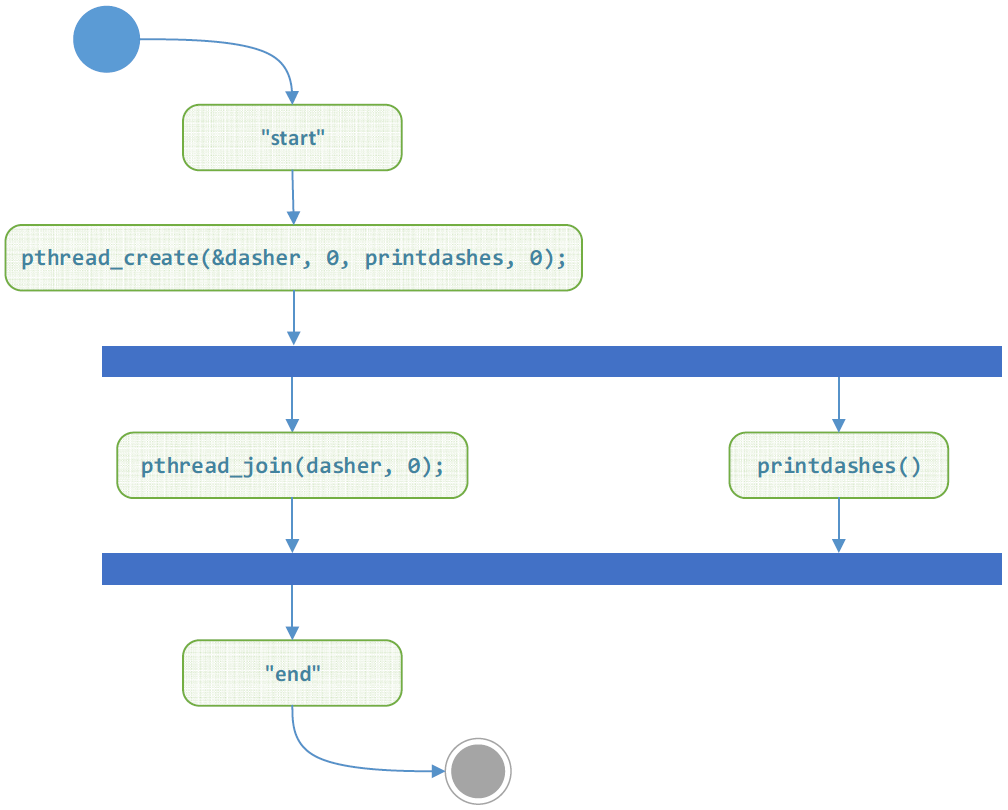
\includegraphics[width=0.8\columnwidth]{images/posix_thread_fork_join.png}
% \end{center}
\begin{minipage}[t]{0.48\columnwidth}
    \lstinputlisting[aboveskip=1mm, firstnumber=1, firstline=1, lastline=23, morekeywords={[3], arg, ret, dasher, i}, morekeywords={[2], pthread_t}]{snippets/posix_join.c}
\end{minipage}
\hfill
\begin{minipage}[t]{0.48\columnwidth}
    \lstinputlisting[aboveskip=1mm, firstnumber=24, firstline=24, lastline=48, morekeywords={[3], arg, ret, dasher, i}, morekeywords={[2], pthread_t}]{snippets/posix_join.c}
\end{minipage}


\subsection{Thread-safeness}
Thread-safeness bezieht sich auf die Fähigkeit einer Anwendung, mehrere Threads gleichzeitig auszuführen,
\textbf{ohne 'clubbering' und 'race conditions'} zu verursachen. Damit Thread-safeness gewährleistet werden kann, ist \textbf{Synchronisation}
erforderlich.

\begin{description}
    \item[clubbering:] Speicher durcheinander bringen, wenn mehrere Threads den gleichen Speicher benötigen und 'falsch' darauf zugreifen
    \item[race conditions:] Programmablauf und Endergebnis hängen davon ab, in welcher Reihenfolge 'gleichzeitig' ablaufende Threads auf z.B. eine
        globale Variable im Speicher zufreifen und das Verhalten somit unvorhersehbar wird
\end{description}


\subsubsection{Empfehlung: Thread-Safeness}

Wenn Thread-safeness nicht explizit garantiert ist (z.B. von einer Library, welche verwendet wird), muss  angenommen werden, dass sie 
\textbf{nicht thread-safe} ist! \\
Um in einem solchen Fall Thread-safeness zu gewährleisten, können die Aufrufe einer 'unsicheren' Funktion \textbf{serialisiert} werden.


\subsection{Quasi-Parallelität / 'Prozess'-Zustände}

\subsubsection{Prozess-Zustände}

\begin{minipage}[t]{0.45\columnwidth}
    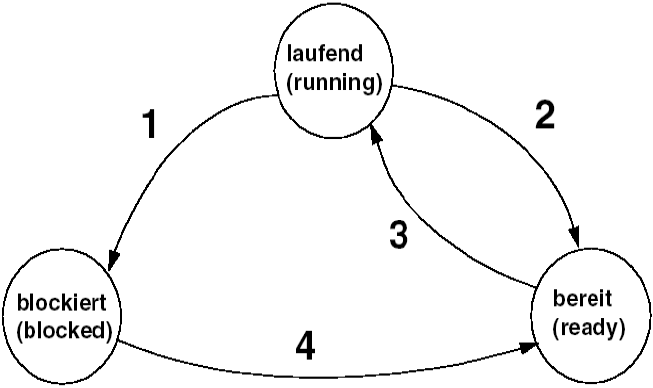
\includegraphics[width=\columnwidth, align=t]{images/posix_process_states.png}
\end{minipage}
\hfill
\begin{minipage}[t]{0.5\columnwidth}
    \begin{enumerate}
        \item I/O Operation, Warten auf Bedingung
        \item Scheduler entzieht CPU
        \item Scheduler weist CPU zu
        \item I/O beendet, Bedigung erfüllt
    \end{enumerate}
\end{minipage}

\vspace{0.2cm}

\begin{minipage}[t]{0.4\columnwidth}
    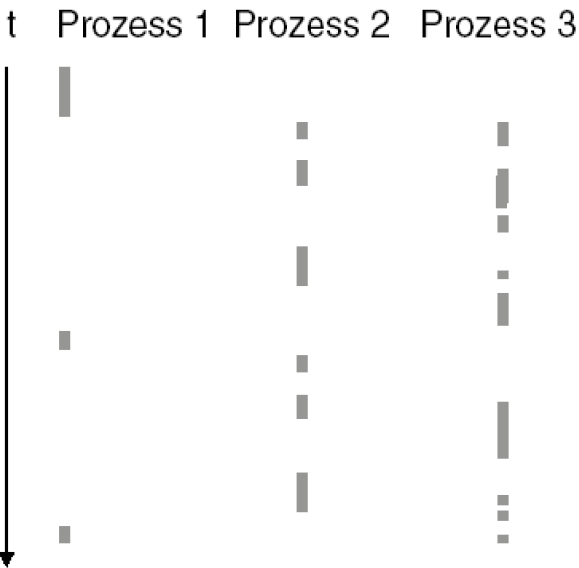
\includegraphics[width=\columnwidth, align=t]{images/concurrency_quasi_parallelitaet.png}
\end{minipage}
\hfill
\begin{minipage}[t]{0.58\columnwidth}
    \raggedright
    \begin{outline}
        \1 Prozesse / Threads warten die 'meiste Zeit' \\
            \textrightarrow\ blocked (z.B. \mylstbox{join} blockiert andere Threads)
        \1 Scheduler ordnet CPU denjenigen Prozess / Thread zu, die im Zustand 'ready' sind und 'etwas zu tun haben'
        \1 Die Zuordnung hängt vom verwendeten Scheduling-Algorithmus ab:
            \2 First come First serve Scheduling: Eine Queue mit allen Prozessen, wobei nächster Prozess jeweils hinten angehängt wird und erster 
                Eintrag der Queue aktuell ausgeführt wird
            \2 Priority Scheduling: Pro Priorität gibt es eine Queue. Abarbeitung je nach Algorithmus anders
    \end{outline}
\end{minipage}


% -------------------------------------------------------------------------------------------------------------------------------------------------
% CHECK: new section?
\subsection{Synchronisation}

Synchronisation wird benötigt, um den \textbf{Zugriff auf gemeinsame Ressourcen} in Critical Sections (CS) zu 'kontrollieren'.


\subsubsection{Defintition: Critical Section (CS)}

\begin{outline}
    \1 Codebereich, in dem nebenläufige oder parallele Prozesse auf gemeinsame Ressourcen zugreifen
        \2 Zu jeder Zeit darf sich \textbf{höchstenns ein Prozess} im kritischen Abschnitt befinden
    \1 Der Exklusive Zugriff durch höchstens einen Prozess wird mittels \textbf{gegenseitigem Ausschluss (Mutex)} sichergestellt
        \textrightarrow\ Siehe Abschnitt \ref{Mutex (mutual exclusion)}
\end{outline}


\subsubsection{Forderungen an die Synchronisation}

\begin{enumerate}
    \item Maximal ein Prozess in einem kritischen Abschnitt (CS)
    \item Über Abarbeitungsgeschwindigkeit, bzw. Anzahl Prozesse dürfen keine Annahmen getroffen werden
    \item Kein Prozess darf \textbf{ausserhalb} eines kritischen Abschnitts einen anderen blockieren
    \item Jeder Prozess, der am Eingang eines kritischen Abshcnitts wartet, muss irgendwann den Abschnitt betreten dürfen 
        (\textbf{fairness condition}) \textrightarrow\ Verhinderung von 'starvation'
\end{enumerate}


% CHECK: new section?
\subsection{Mutex (mutual exclusion)}
\label{Mutex (mutual exclusion)}

Die Lösungsstruktur 'Mutex' (gegenseitiger Ausschluss) stellt sicher, dass höchstens ein Prozess auf eine Critical Section (CS) zugreift. 


\subsubsection{Mutex -- Ablauf}

\begin{minipage}[c]{0.62\columnwidth}
    \raggedright

    \begin{description}
        \setlength\itemsep{2em}
        \item[Zugriffsprüfung:] Warten bis der Zugang frei wird
        \item[Sperren:] Signal wird für andere auf Rot gesetzt, damit nur ein Prozess im kritischen Abschnitt sein kann
        \item[Freigeben:] Rotes Signal wird wieder gelöscht
    \end{description}
\end{minipage}
\hfill
\begin{minipage}[c]{0.37\columnwidth}
    \begin{center}
    \begin{tikzpicture}
        [
            %transform canvas={scale=1.0},
            scale = 0.7,
            >=latex,
            bluebox/.style={rectangle, draw=black, fill=blue!40, thick, minimum width=1.5cm, minimum height=0.6cm, align=center},
            redbox/.style={rectangle, draw=black, fill=redcontrast!70, text=white, thick, minimum width=1.5cm, minimum height=0.6cm, align=center},
        ]
        % define styles
        
        % nodes
        \node[bluebox]      (Zugriff)                                               {Zugriff\\erlaubt?};
        \node[bluebox]      (Sperren)           [below= 0.4cm of Zugriff]           {Sperren};   
        \node[redbox]       (CS)                [below= 0.3cm of Sperren]           {kritischer\\Abschnitt};
        \node[bluebox]      (Freigeben)         [below= 0.3cm of CS]                {Freigeben};
        
        \node               (wait)              [right= 0.2cm of Sperren]           {\lstinline|waitFor(signal)|};
        \node               (send)              [right= 0.2cm of Freigeben]         {\lstinline|send(signal)|};
        
        % arrows between nodes
        \draw[->, thick] (Zugriff.south)    to (Sperren.north);
        \draw[->, thick] (Sperren.south)    to (CS.north);
        \draw[->, thick] (CS.south)         to (Freigeben.north);
    \end{tikzpicture}
\end{center}
\end{minipage}


\subsubsection{Verwendung von Signalen und Semaphoren}

\begin{outline}
    \1 Jeder Prozess wartet vor dem Betreten der CS auf ein gemeinsames Signal
        \2 Wenn das Signal gesetzt ist, ist CS frei
        \2 Mehrere Prozesse können gleichzeitig warten \textrightarrow\ Schedulingalgorithmus bestimmt 'nächsten' Thread 
    \1 \mylstbox{waitFor(signal)} blockiert \textbf{aufrufenden} Prozess, falls Signal nicht gesetzt
    \1 Jeder Prozess, der fertig ist, setzt das Signal mit \mylstbox{send(signal)}
\end{outline}


\para{Semaphoren}

\begin{outline}
    \1 'Semaphor' ist ein spezieller Name für ein Signal für den \textbf{Zutritt zu einer CS}
    \1 Es gibt zwei atomare (nicht unterbrachbare) Operationen auf einer Semaphoren \lstinline|s|
        \2 Passieren P(s): Beim Eintritt in CS \textrightarrow\ \mylstbox{waitFor(s)}
        \2 Verlassen V(s): Beim Austritt aus CS \textrightarrow\ \mylstbox{send(s)}
\end{outline}

\vspace{0.2cm}

Bei der Verwendung von Semaphoren treten folgende Probleme auf

\vspace{0.1cm}

\begin{outline}
    \1 Ressourcen können besetzt bleiben, wenn V(s) vergessen wird
        \2 \textbf{Für jedes P(s) braucht es auch ein V(s)}
    \1 Grössere Programme: Es können subtile Probleme entstehen, falls z.B. das V(s) in einer \textbf{if-Bedingung} gemacht wird
    \1 Beim Auftreten von Exceptions kann das Freigeben schwierig werden
\end{outline}

\vspace{0.1cm}

\textrightarrow\ Lösung für das Freigabe-Problem: RAII (siehe Abschnitt )   % TODO Ref to section when available


\subsubsection{Busy Waiting}

\begin{outline}
    \1 Prozesse warten \textbf{aktiv} in einer Schleife (\textbf{spin lock})
        \2 Wartende Prozesse \textbf{belasten} unnötigerweise den Prozessor
\end{outline}

\vspace{0.1cm}

Die Lösung für Busy Waiting ist, die wartenden Prozesse in eine \textbf{Warteschlange} einzutragen (\textbf{sleep and wakeup})


% CHECK New section?
\subsection{Thread Synchronisierung in C mit pthreads API}

Code Synchronisation wird mittels Mutex (\textbf{lock pattern}) sichergestellt. 
Das Konzept von Mutex ist, dass eine Mutex Variable \textbf{nur einem Thread gleichzeitig gehören kann.}


\subsubsection{Ablaub einer Mutex-Sequenz in C}

\begingroup
\renewcommand{\outlinei}{enumerate}
\renewcommand{\outlineii}{itemize}
\begin{outline}
    \1 Mutex Variable erstellen / instanzieren
        \2 'Schloss', welches Zugang zu CS schützt
    \1 Mehrere Threads versuchen, die Mutex Variable zu blockieren \\
        \textrightarrow\ \textbf{Nur ein Thread} ist erfolgreich \textrightarrow\ diesem Thread ('owner') gehört die Mutex Variable 
    \1 Dieser 'owner thread' führt Aktionen in der Critial Section (CS) aus
        \2 Häufig Update einer globalen (shared) Variable
    \1 'owner' entblockt (unlock) die Mutex Variable
    \1 Dem nächsten Thread gehört die Mutex Variable \textrightarrow\ zurück zu Schritt 2
    \1 Wenn alle Threads abgearbeitet sind, wird die Mutex Variable zerstört
\end{outline}
\endgroup

\vspace{0.1cm}

\textrightarrow\ Dies ist ein sicherer Weg, um sicherzustellen, dass, wenn \textbf{mehrere Threads} dieselbe Variable aktualisieren, 
der \textbf{Endwert derselbe} ist, wie wenn nur \textbf{ein Thread} die \textbf{Aktualisierung durchführen} würde.


\example{Mutex in C}

\lstinputlisting[aboveskip=1mm, belowskip=0mm,
                 morekeywords={[3], val , valMtx, arg, t1, t2, rState}, morekeywords={[2], pthread_mutex_t, pthread_t}]
                {snippets/posix_mutex.c}



\subsection{Monitorprinzip (Monitor Pattern)}

% CHECK: ob diese Aussage korrekt ist...
Das Monitorprinzpt beschreibt eine Art Abstraktion des Mutex / Lock Patterns. \\
Dabei muss sich der \textbf{Aufrufer nicht mehr um die Synchronisation der Threads kümmern}. Das Problem wird einmal im Monitor gelöst.

\begin{outline}
    \1 Es wird ein Abstrakter Datentyp (ADT) definiert, der genau die Funktionen in der Schnittstelle anbietet, die notwendig sind
    \1 Der Aufrufer ruft diese Funktion auf, muss sich aber \textbf{nicht um Synchronisation kümmern}
        \2 Synchronisation (z.B. mit Semaphoren) ist Implementation des Monitors lokal gelöst
\end{outline}


\subsection{'Stolperfallen' bei Synchronisation}
% TODO: Besserer Name...

\subsubsection{Starvation (Verhungern)}

\begin{outline}
    \1 Zustand, bei dem ein Prozess nie dran kommt \textrightarrow\ er verhungert
    \1 Kann auftreten bei:
        \2 prioritätsgetriebenen Systemen bei Prozessen mit niederer Priorität passieren
        \2 SJF (shortest job first) Systeme \textrightarrow\ kurze Jobs bremsen längere Jobs aus
    \1 Fairness condition besagt, dass Starvation verhindert werden muss
\end{outline}


\subsubsection{Deadlock}

\begin{outline}
    \1 Situation, bei der sich \textbf{zwei Prozesse gegenseitig blockieren}
        \2 Zwei Prozesse benötigen gemeinsame Ressourcen A und B. Wenn Prozess 1 die Ressource A bereits besitzt und Prozess 2 die Ressource B,
            dann warten beide unendlich lange auf die jeweils andere Ressource
\end{outline}

\vspace{0.1cm}

\textbf{Deadlock kann vermieden werden, indem alle Prozesse die gemeinsamen Ressourcen immer in
\myul{derselben Reihenfolge} anfordern (z.B. zuerst A, dann B)}



\subsection{Informationen zwischen Threads austauschen}

Der Austauschen von Daten zwischen verschiedenen Threads (z.B. anderen Thread benachrichtigen, wenn in eigenem Thread etwas passiert ist / warten,
bis in anderem Thread etwas passiert ist ) ist mittels \textbf{shared resources} möglich. \\
Der \textbf{Nachteil} davon ist aber, dass diese shared resource mit \textbf{polling} abgefragt werden muss \textrightarrow\ nicht effizient!

\vspace{0.1cm}

Der korrekte Weg für den Informations-Austausch zwischen Threads sind \textbf{condition variables.}


\subsubsection{Condition Variables}

\begin{outline}
    \1 Mit Hilfe von condition variables können Threads auf der Grundlage des aktuellen Datenwerts synchronisiert werden
        \2 \textbf{Kein polling nötig!}
    \1 Condition Variables werden immer \textbf{zusammen mit einem 'Mutex lock'} verwendet
\end{outline}


\example{Anwendungsbeispiel für Condition Variables}

\begin{center}
    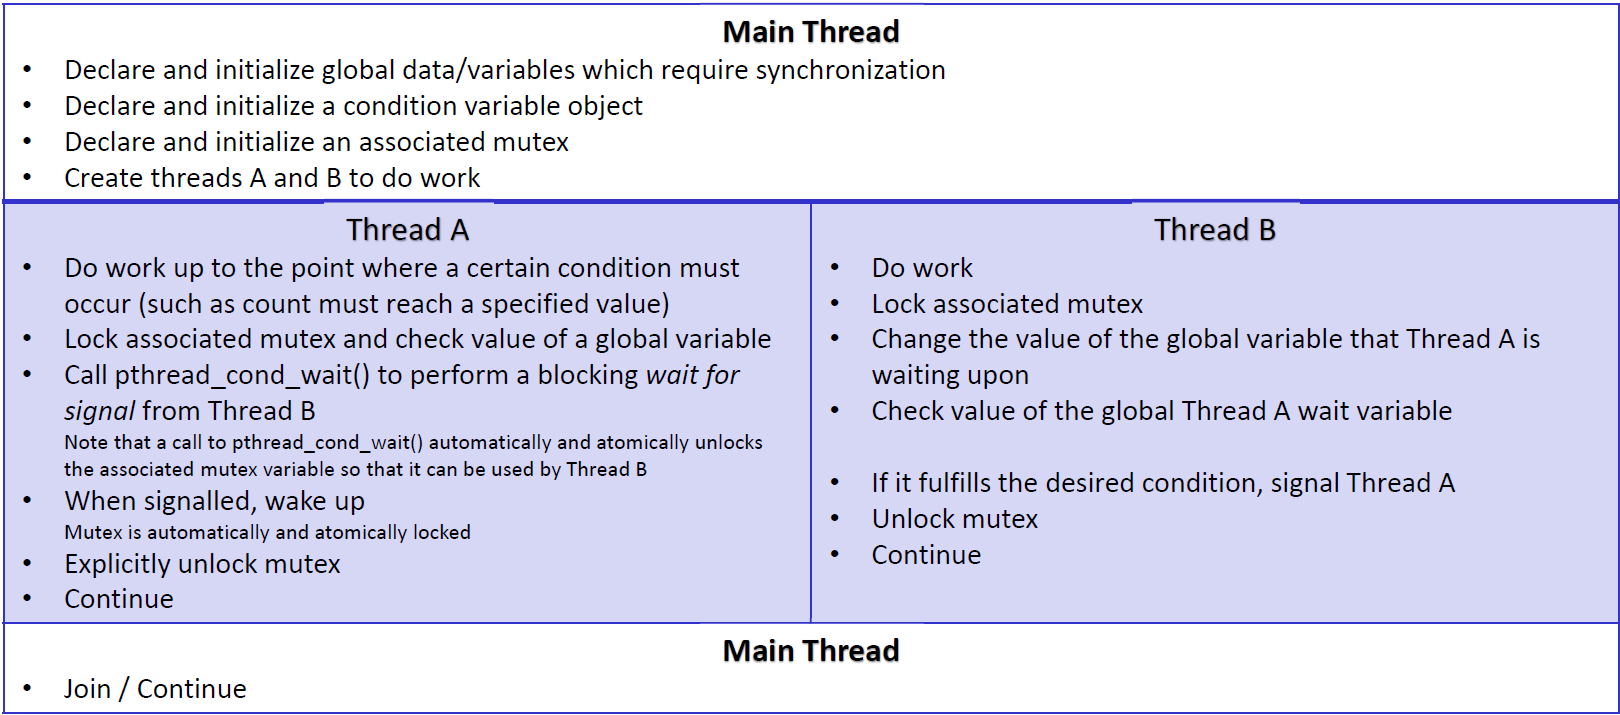
\includegraphics[width=0.9\columnwidth]{images/cond_var_beispiel.png}
\end{center}


\subsection{Condition Variables mit pthreads}

\subsubsection{Erstellen / inizialisieren von Conditon Variables}

\lstinputlisting[aboveskip=0mm, belowskip=0mm, firstnumber=1, firstline=1, lastline=5,
                 morekeywords={[3], condVar, attr}, morekeywords={[2], pthread_cond_t, pthread_condattr_t}]
                {snippets/posix_condition_variables_interface.c}


\subsubsection{Zerstören von Condition Variables}

\lstinputlisting[aboveskip=0mm, belowskip=0mm, firstnumber=1, firstline=8, lastline=9,
                 morekeywords={[3], condVar}, morekeywords={[2], pthread_cond_t}]
                {snippets/posix_condition_variables_interface.c}


\subsubsection{Auf Conditon Variables warten}

% TODO S 10


\lstinputlisting[aboveskip=0mm, belowskip=0mm, firstnumber=1, firstline=12, lastline=14,
                 morekeywords={[3], condVar, mutex}, morekeywords={[2], pthread_cond_t, pthread_mutex_t}]
                {snippets/posix_condition_variables_interface.c}


\subsubsection{Signalisierung mit Conditon Variables}

% TODO: 11 
\lstinputlisting[aboveskip=0mm, belowskip=0mm, firstnumber=1, firstline=17, lastline=18,
                 morekeywords={[3], condVar}, morekeywords={[2], pthread_cond_t}]
                {snippets/posix_condition_variables_interface.c}